%!TEX root = tesis.tex


\chapter{Un \ssolver paralelo y distribuido }
\label{ssolver-pardist}

La implementación de nuestra herramienta como un sistema distribuido persigue
el objetivo fundamental de mejorar el tiempo de ejecución ya sea decrementando
el tiempo necesario para resolver un determinado problema o transformando un
problema previamente irresoluble (en tiempo razonable) en resoluble. Para ello
el sistema debe ser \textbf{escalable} en tanto que debe tener la capacidad de
incorporar mayor cantidad de \hard a la resolución del problema. Por otro
lado, el uso de este \hard debe ser \textbf{eficiente} en el sentido de que la
utilización de mayor cantidad de \hard debe resultar en un incremento de la
performance del sistema (en nuestro caso entendida como se describió
previamente).

\begin{wrapfigure}{R}{0.4\textwidth}
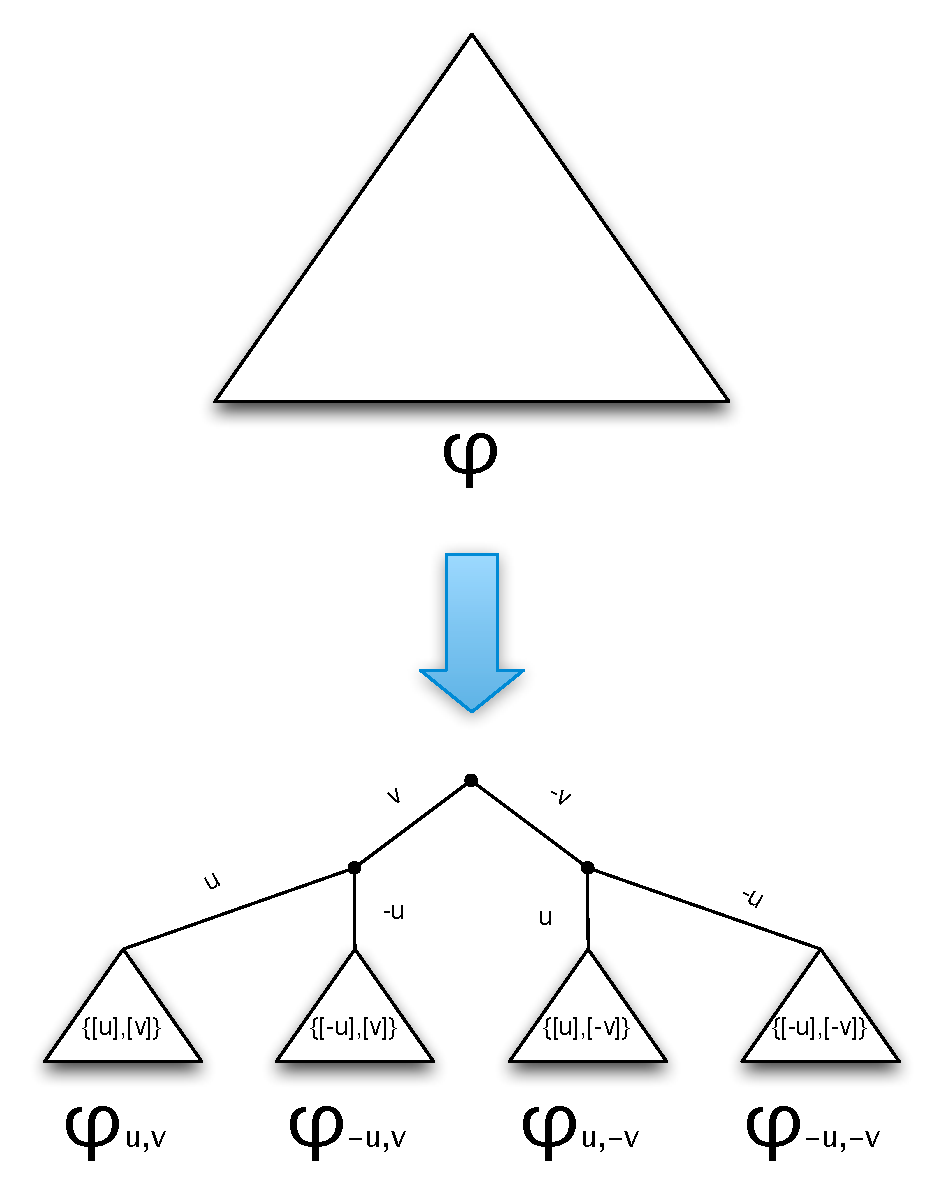
\includegraphics[scale=0.4]{graphs/split por guiding path}
\caption{Esquema de partición por \gp}
\label{fig:guidingpaths}
\end{wrapfigure}

Con estos dos objetivos en mente desarrollamos una \ssolver distribuido basado
en la idea de \gp y orienteado a \clusters de computadoras. La idea de \gp se
basa en la observación de que, en el peor caso, todas las posibles valuaciones
de una fórmula proposicional $\varphi$ deben ser evaluadas. Una vez que una
valuación que satisface a una fórmula es encontrada, el procedimiento de
\ssolving puede ser abortado\footnote{Existe otra variante en la que, además
de determinar si una fórmula es \sat o \unsat, interesa enumerar todos los
posibles modelos de dicha fórmula. En este escenario el procedimiento de
\ssolving no puede ser detenido una vez que se encuentra una valuación sino
que el mismo debe continuar hasta agotar todas las posibles valuaciones que
satisfacen a la fórmula en cuestión.}. Por el contrario, si la fórmula es
\unsat, la única alternativa para poder asegurarlo es agotar todas las
posibles valuaciones y determinar que ninguna de ellas satisface a la fórmula
en cuestión. Por lo tanto, una forma de dividir el problema es tomar una
variable $v$ y construir los dos subproblemas $\varphi_{v \leftarrow 0}$ y
$\varphi_{v \leftarrow 1}$ que se derivan de las dos posibles asignaciones de
valores de verdad a dicha variable. Una vez hecho esto, determinar que el
problema original $\varphi$ es \unsat se reduce a determinar que tanto
$\varphi_{v \leftarrow 0}$ como $\varphi_{v \leftarrow 1}$ son \unsat. Por el
contrario, determinar que el problema es \sat reduciría a establecer que
$\varphi_{v \leftarrow 0}$ es \sat o bien que $\varphi_{v \leftarrow 1}$ lo
es. Ahora, $\varphi_{v \leftarrow 0}$ y $\varphi_{v \leftarrow 1}$ pueden ser
considerados como dos problemas independientes y volver a aplicar la misma
idea recursivamente. Naturalmente este proceso puede realizarse seleccionando
más de una variable en cada paso. Al seleccionar $n$ variables obtendremos
entonces $2^n$ subproblemas. Llamaremos \emph{levantar variables} al proceso
de dividir un problema $\varphi$ en los $2^n$ subproblemas que resultan de
aplicar todas las posibles valuaciones sobre el conjunto de $n$ variables
levantadas. Se desprende de esto que una de las tareas que debe poder cumplir
la herramienta es la de dividir un problema.

% El objetivo principal de todo sistema distribuido es que el mismo sea
% \textbf{escalable}. Si bien la escalabilidad puede ser entendidad en
% diferentes sentidos, nos interesa en particular que el sistema haga posible la
% utilización de mayor cantida de \hard para resolver el problema (en nuestro
% caso un problema \sat) y que esa utilización de mayor poder de cómputo reporte
% ganancias en términos de tiempo (percibido) invertido en resolver un
% determinado problema o bien en términos de empujar la frontera de lo
% resoluble.

La escalabilidad como gran objetivo rector en el desarrollo de nuestra
herramienta introduce una serie de desafíos, a saber:
\begin{itemize}
	\item Almacenamiento distribuido.
	\item Simetría de capacidades en los nodos de trabajo (\ws).
	\item Minimización de la utilización de la red de comunicaciones.
\end{itemize}

La necesidad de que el almacenamiento de problemas pendientes de resolución se
encuentre distribuido se debe a un doble aspecto. Por un lado, la cantidad de
subproblemas producidos puede ser muy grande. Por lo tanto no es viable
requerir que la cantidad de espacio necesario para almacenar todas las tareas
pendientes de resolución se encuentre disponible en una misma ubicación. Aún
cuando fuera posible tener la cantidad de espacio necesaria para almacenar
todos los subproblemas en una ubicación centralizada surge un segundo problema
que presentaría este enfoque que es el de la contención. En este aspecto, si
pretendemos que el almacenamiento no se vuelva un cuello de botella es vital
distribuir las tareas pendientes de modo que cuando los \ws requieran nuevas
tareas para resolver, los múltiples pedidos no recaigan en un mismo equipo.

El requisito de que los nodos de trabajo (\ws) sean simétricos se desprende de
la necesidad de eliminar los cuellos de botella. La simetría entendida en su
máxima expresión como la posibilidad de que todas las unidades de
procesamiento puedan realizar todas las funciones necesarias provee la
capacidad de distribuir la carga de trabajo de la manera más conveniente en
cada momento. Esto no podría ser logrado si los nodos de trabajo tuvieran
funciones específicas ya que se podría dar el caso de tener nodos ociosos
porque no hay trabajo pendiente de la clase de trabajo que esos nodos saben
realizar mientras que al mismo tiempo tendríamos nodos sobrecargados. Esta
situación podría empeorar seriamente a medida que la cantidad de nodos
aumenten.

En nuestro caso particular, el requisito de simetría se traduce en que los \ws
deben poseer las capacidades de: \begin{inparaenum}[a)] \item \solvear
\todo{buscar una forma de decir esto que no sea tan fea o en su defecto
definir esto en la parte de preliminares} un subproblema (consumir), \item
dividir un subproblema en nuevos subproblemas (producir) y \item almacenar,
solicitar y transferir subproblemas (distribuir). \end{inparaenum}

Además de los desafíos de escalabilidad, surgen también los desafíos
relacionados con la eficiencia o la performance de la herramienta. Entre ellos
los más destacados son:

\begin{itemize}
	\item Movilidad de tareas.
	\item Crecimiento a la par de los \ssolvers secuenciales.
	\item No hacer burradas \todo{Revisar toda esta itemización. No me convence....}
\end{itemize}

El triple rol de productor, consumidor y distribuidor asignado a los \ws hace
que la movilidad de tareas se transforme en un desafío en tanto que un \w
puede estar \solveando al mismo tiempo que otro \w le solicita una tarea
pendiente. Es evidente que en esta situación no es viable que el \w que está
esperando una tarea tenga que esperar a que el \w que tiene dicha tarea
termine de \solvear para que su pedido sea completado.

Otro de los objetivos que perseguimos a la hora de diseñar nuestra herramienta
fue que la misma pudiera utilizar un \ssolver \ots para la resolución local de
un subproblema. Esto nos permite aprovechar los avances que se han obtenido en
el área de \ssolving secuencial en los últimos años (que han sido muchos) a la
vez que nos permite, a futuro, evolucionar a la par de los \ssolvers
secuenciales de manera más simple. Esto proporciona la posibilidad de que la
herramienta no se vuelva obsoleta ante un nuevo avance en el campo de
\ssolving secuencial.

\newcommand{\rt}{\emph{run-time}\xspace}
\newcommand{\apriori}{\emph{a priori}\xspace}

Generar una estrategia automática que proporcione buenos resultados en la
ejecución de problemas diversos es sumamente difícil. Más aún, no tener la
posibilidad de modificar la estrategia adoptada durante una corrida (que puede
ser sumamente larga y con características desconocidas \apriori) puede tener
resultados catastróficos. Esto nos motivó a adoptar un enfoque en el que la
maquinaria de cómputo distribuido no posee inteligencia alguna y por el
contrario provee una serie de funciones básicas que pueden ser invocadas
remotamente. La operación del sistema por lo tanto se lleva a cabo desde un
\textbf{tablero de control} que permite al usuario manipular el sistema de
cómputo en \rt.

\

\noindent\underline{\textbf{Nota sobre la implementación}}

\

El último objetivo que perseguimos durante el desarrollo de nuestra
herramienta fue que la misma presentara facilidad para ser modificada sin que
esto impacatar negativamente en la \emph{performance}. Este objetivo, entre
otras cosas, determinó la elección de las tecnologías a utilizar para su
desarrollo. Por lo tanto se utilizó el lenguaje de programación \Python para
el desarrollo de toda la herramienta con excepción de la parte de cómputo
intensivo. Al utilizar un \ssolver \ots no fue necesario elegir un lenguaje
para su desarrollo. En la implementación actual de la herramienta utilizamos
el \ssolver \minisatdosveinte que está desarrollado en el lenguaje \cpp. Para
ello se desarrolló un \emph{wrapper} que permite utilizar \minisat desde un
entorno \Python. Para el intercambio de mensajes entre los \ws se utilizó el
estándar \mpi a través de la biblioteca \texttt{mpi4py}\cite{mpi4py}.


% \begin{itemize}
% 	\item Escalable
% 	\item Uso de SAT Solver off-the-shelf
% 	\item Multiplataforma
% 	\item Tablero de control
% \end{itemize}

\section{Arquitectura}

\newcommand{\fig}{Fig.-}

La \fig\ref{fig:arquitectura} muestra la arquitectura de la herramienta. En
la misma se distinguen claramente dos componentes: el \bend que ejecuta sobre
un \cluster de computadoras y el \fend que ejecuta en un equipo que se
encuentra posiblemente fuera del centro de cómputos.

\begin{wrapfigure}{R}{0.45\textwidth}
\fbox{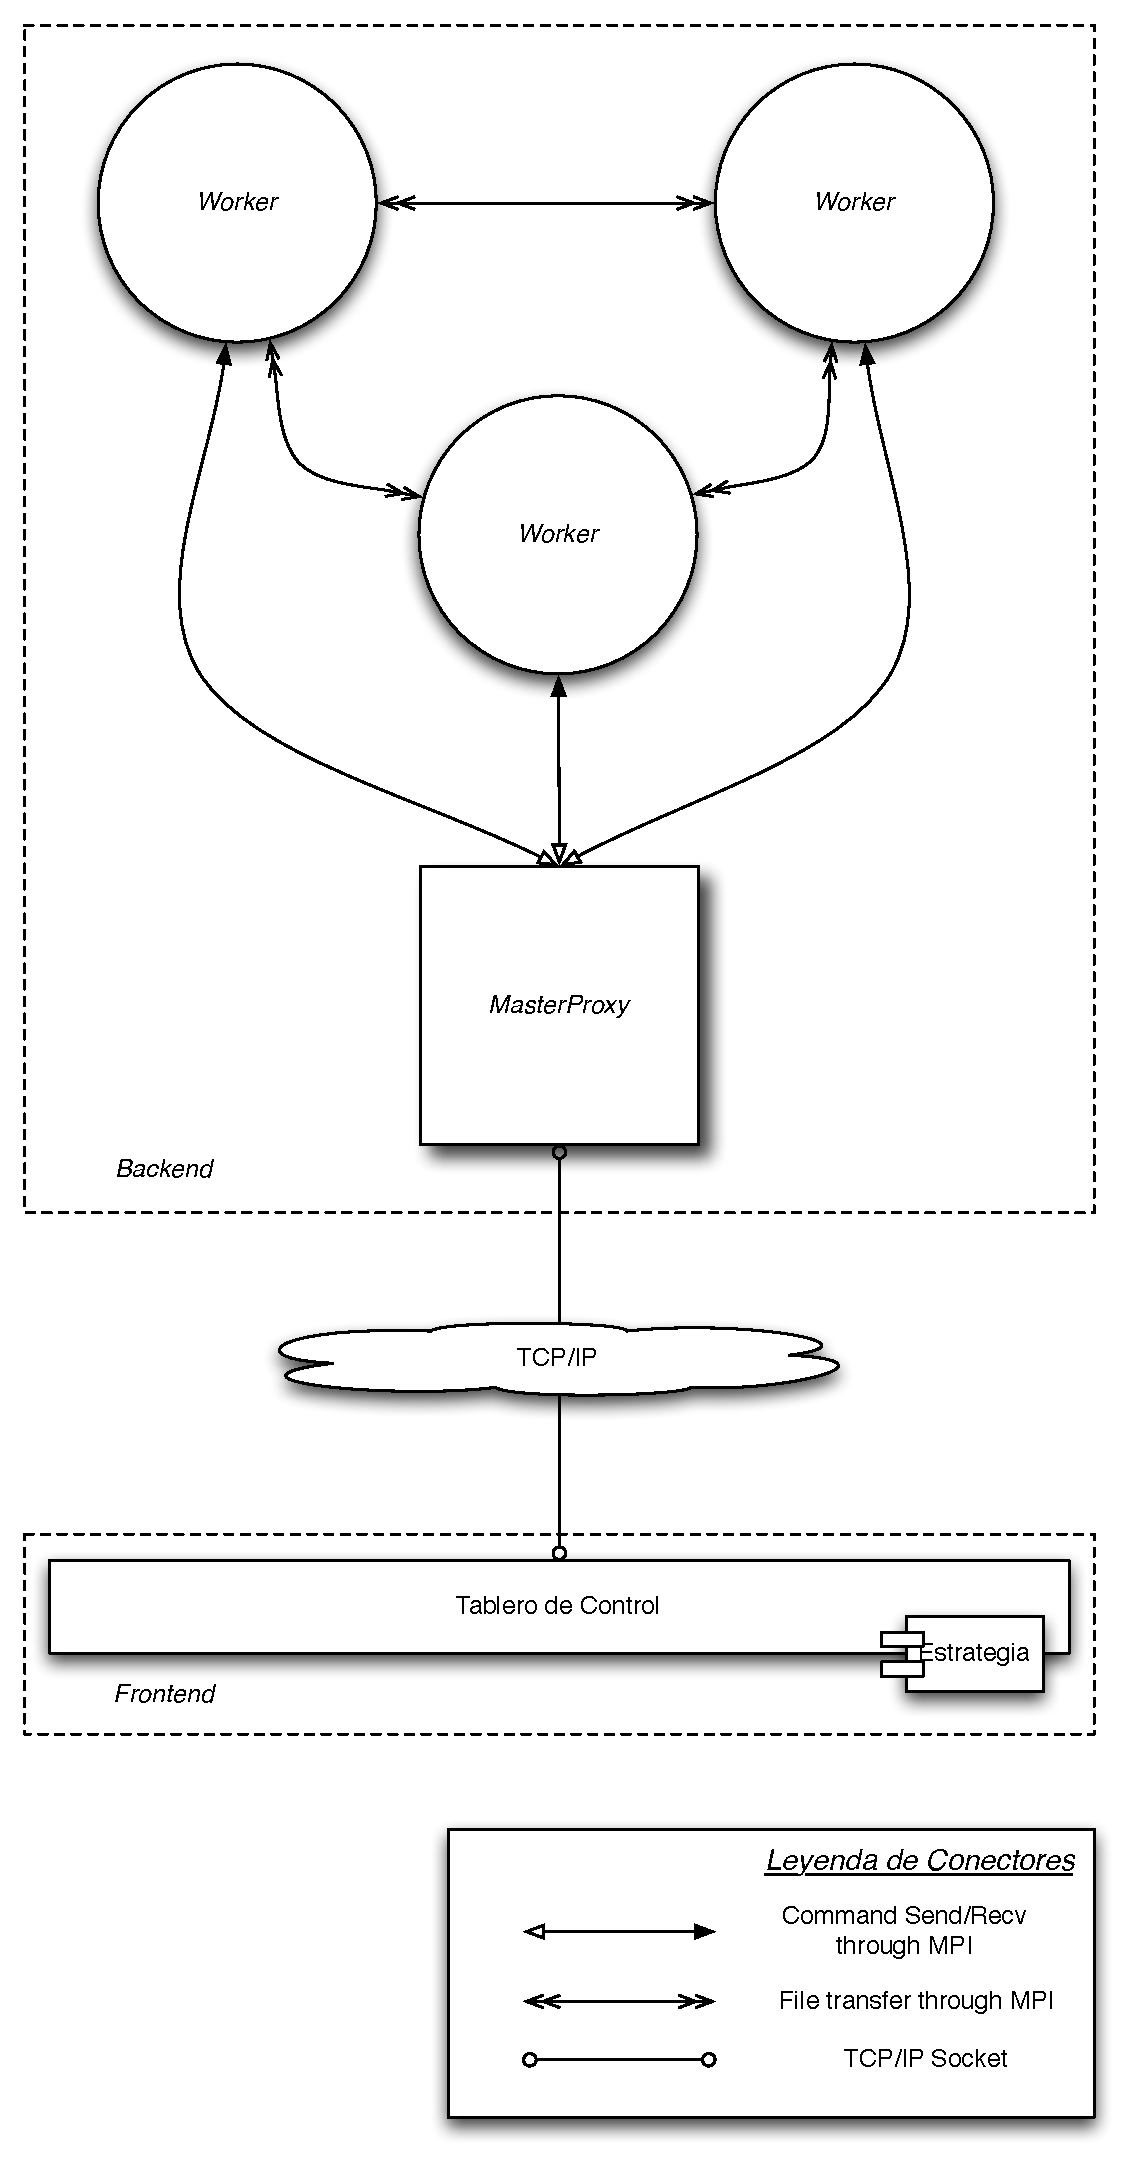
\includegraphics[scale=0.3]{graphs/paralloy architecture}}
\caption{Diagrama de componentes y conectores del \ssolver distribuido}
\label{fig:arquitectura}
\end{wrapfigure}

\subsection{\bend}
\label{sec:backend}
\newcommand{\master}{\emph{MasterProxy}\xspace}

En el \bend se puede observar que existen dos clases distintas de elementos.
Por un lado tenemos un proceso llamado \master que es el encargado de manejar
la comunicación de órdenes desde el \fend hacia los \ws y de reenviar las
respuestas correspondientes desde los \ws hacia el \fend.

En segunda instancia encontramos otro de tipo de procesos, los \ws. Los \ws
son los encargados de relizar el cómputo (\ssolving) y la división de un
problema en nuevos subproblemas. Asimismo son quienes almacenan las tareas
pendientes de ejecución y por lo tanto deben proveer acceso a dicho
almacenamiento a los demás \ws.

\newcommand{\masterslave}{\texttt{Master-Worker}\xspace}

Es importante destacar que si bien el \bend presenta una arquitectura
\masterslave, el \master en este caso no toma ninguna decisión sino que
simplemente actúa como intercambiador de mensajes entre el ambiente externo
(el \fend) y el ambiente interno.

\begin{figure}[h!]
\centering
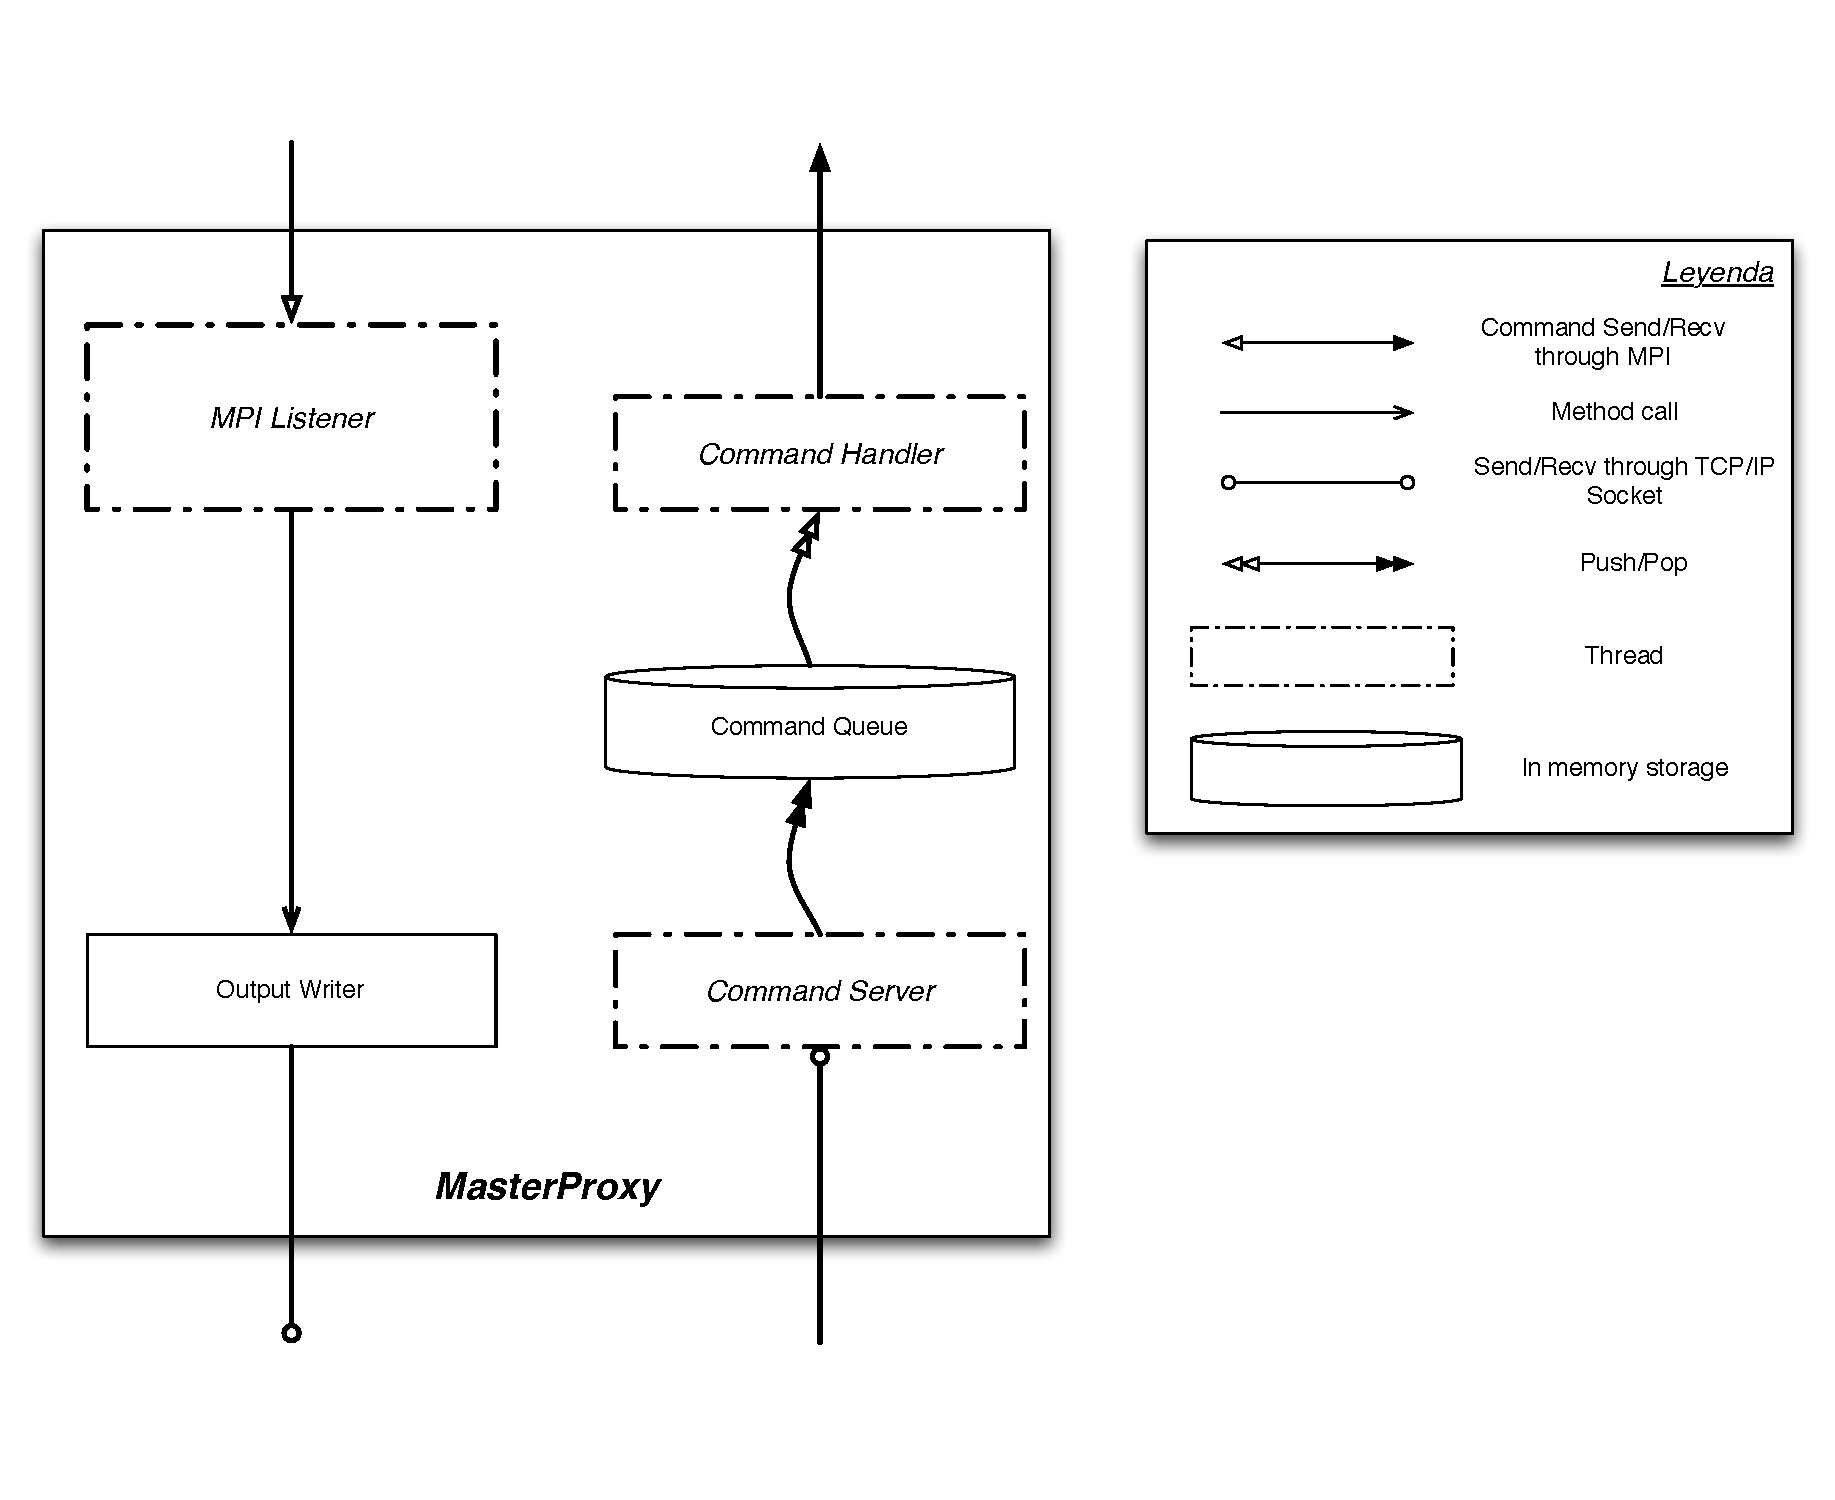
\includegraphics[scale=0.4]{graphs/master proxy detail}
\caption{Detalle de arquitectura del componente \master}
\label{fig:masterproxydetail}
\end{figure}

La \fig\ref{fig:masterproxydetail} detalla la arquitectura del \master. En el
diagrama se puede observar que el \datapath de entrada (\fend hacia \bend) y
el de salida (\bend hacia \fend) son independientes. Esto es una consecuencia
directa que se desprende de la ausencia de inteligencia en el \master. Esto
implica que no es necesario mantener el estado del sistema ya que en este
componente no se toman decisiones. La ausencia de estado hace que el proceso
\master consuma un mínimo de recursos.

La intervención de dos \threads distintos en el \datapath de entrada
proporciona un alto nivel de respuesta ya que permite que algunos comandos
sean implementados internamente mediante comunicación sincrónica a través de
\mpi sin que esto implique una pausa en el procesamiento del flujo de datos de
entrada desde el \fend hacia el \bend. La comunicación sincrónica permite
simplificar algunos comandos como el envío del problema original hacia todos
los \ws. Al mismo tiempo se mantiene el orden entre los comandos enviados
desde el \fend lo cual también contribuye a la simplificación del modelo de
cómputo a pesar de tratarse de un sistema distribuido.

\begin{figure}[h!]
\centering
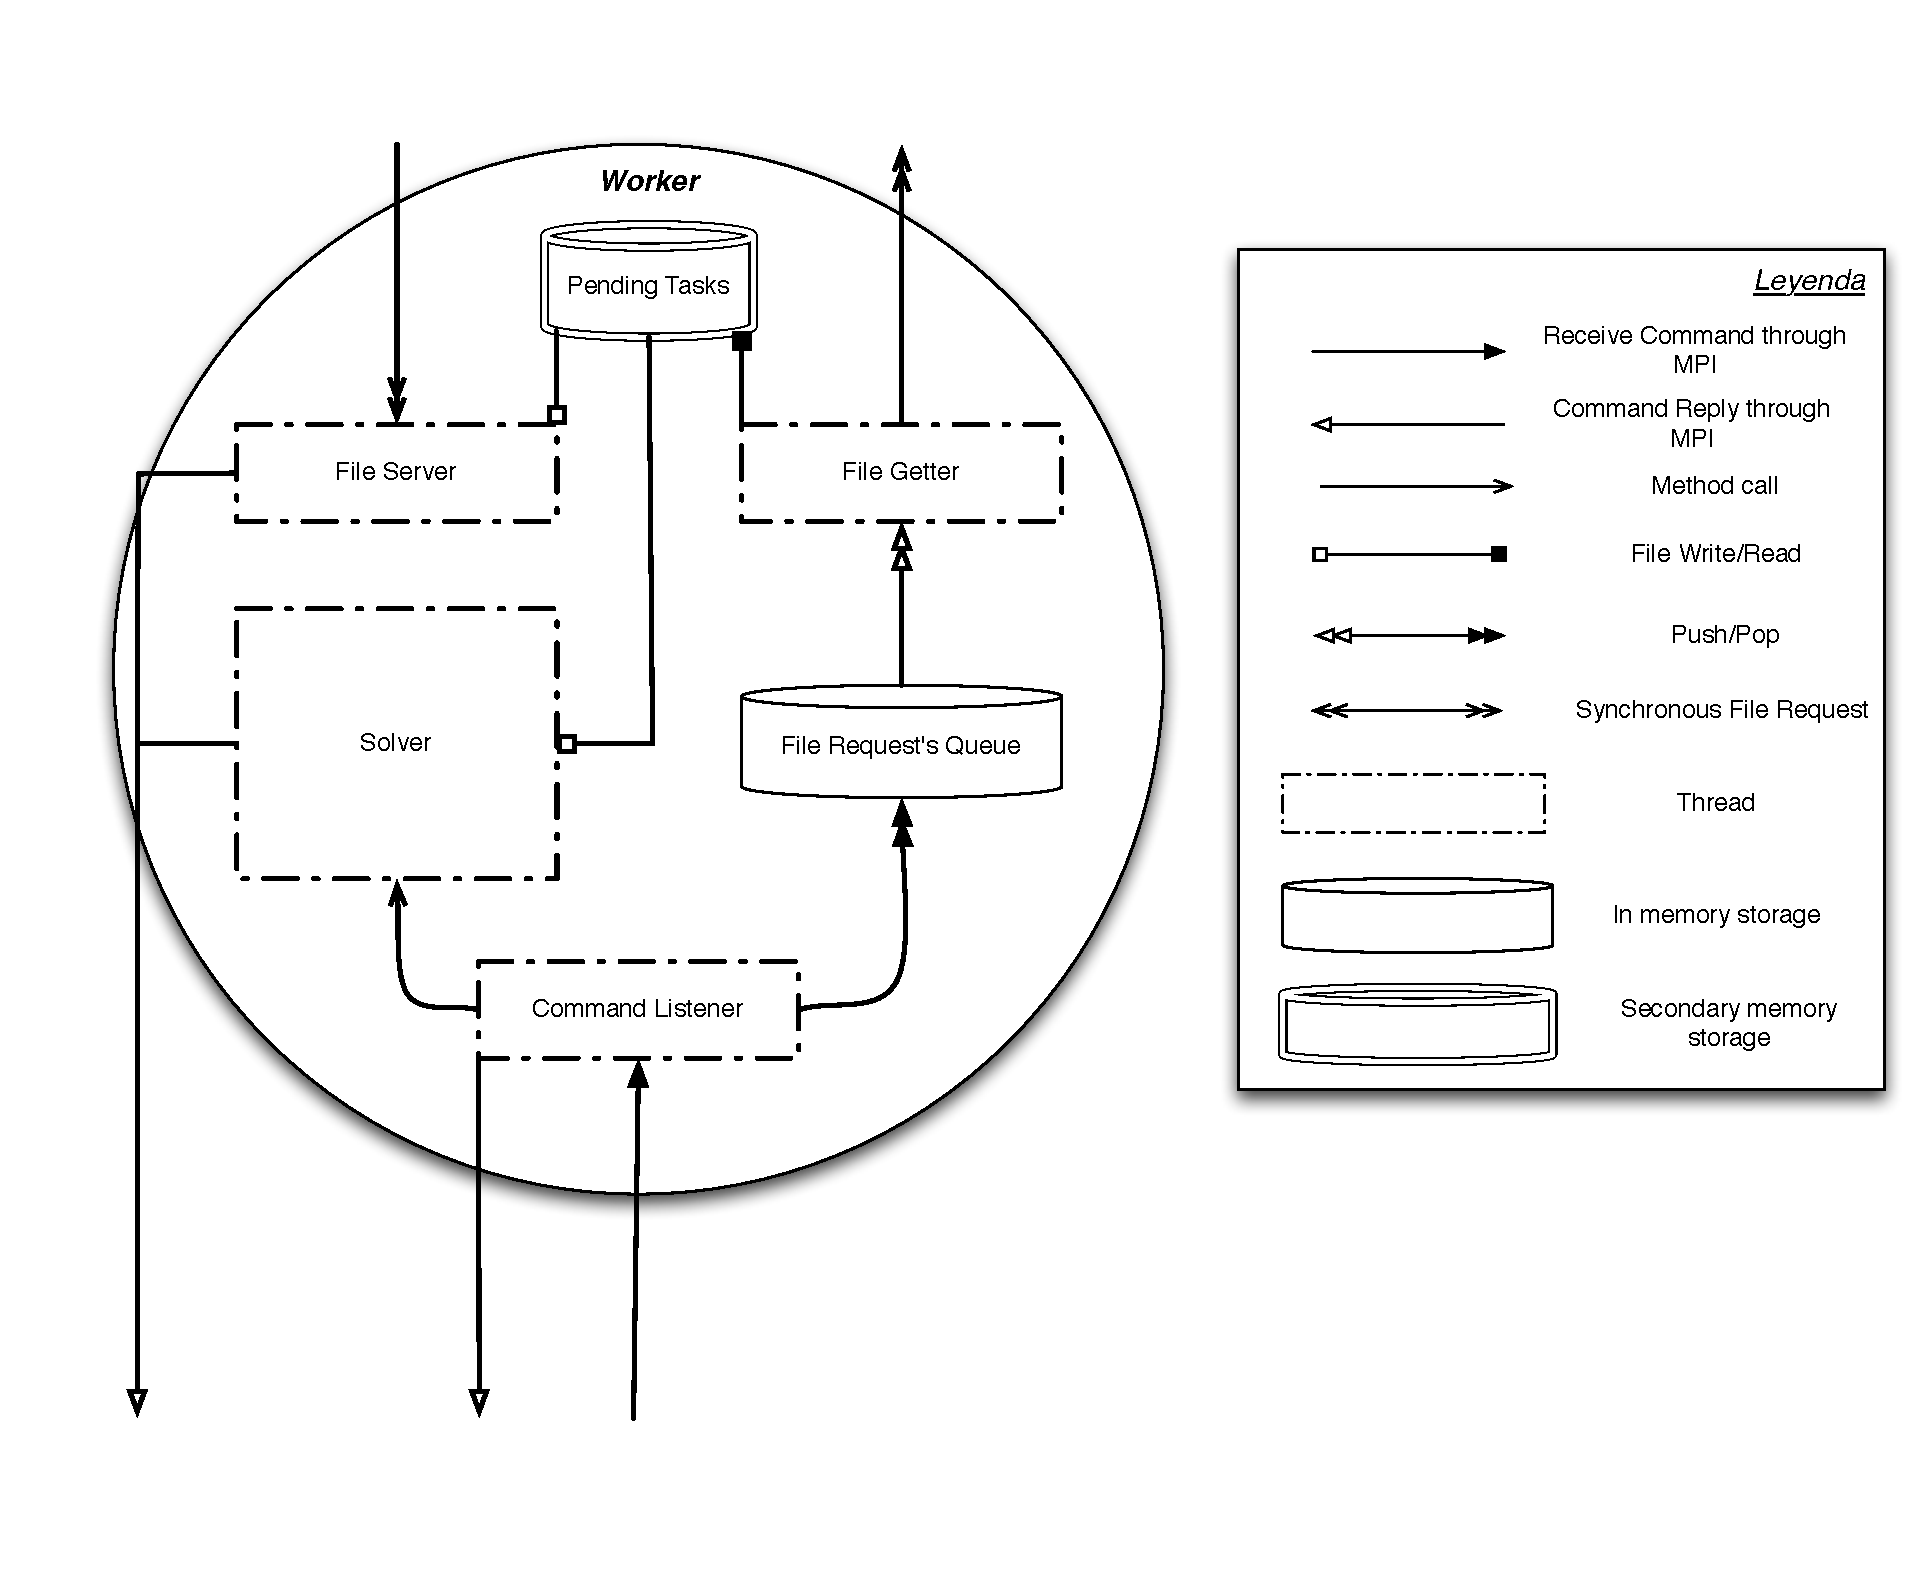
\includegraphics[scale=0.4]{graphs/worker detail}
\caption{Detalle de arquitectura del componente \w}
\label{fig:workerdetail}
\end{figure}

La \fig\ref{fig:workerdetail} muestra el detalle de diseño del componente
\w. Como se puede observar, las funciones de \solving, comunicación y
transferencia de archivos se implementaron en \threads separados. Dado que la
función de \solving utiliza principalmente tiempo de \cpu, mientras que el
resto de las funciones consumen principalmente tiempo de \io, la separación de
éstas en distintos \threads permite la ejecución concurrente de estas
tareas sin que esta característica impacte negativamente en el desempeño del
\ssolver. A la vez, esta característica permite satisfacer el objetivo de
movilidad de las tareas, aún cuando el \w se encuentre ocupado \solveando.

Interesa destacar también que tanto la estrategia de partición de un problema
como la estrategia de aprendizaje se encuentran implementadas en los \ws. Si
bien este diseño es contrario a la idea general de \emph{tablero de control}
consideramos que el nivel de granularidad necesario para poder controlar
remotamente la realización de estas dos tareas era demasiado alto y atentaba
contra la usabilidad de la herramienta. Asimismo, la herramienta es capaz de
poseer diversas estrategias implementadas para estas dos fases de la ejecución
de modo que el usuario puede seleccionar la estrategia deseada (y sus
parámetros en caso que corresponda) desde el \fend.

Por último corresponde mencionar a qué nos referimos en concreto cuando
hablamos de \emph{tarea}. El término \emph{tarea} fue mencionado en varias
ocasiones a lo largo de la explicación. Si bien conceptualmente una tarea
podría ser simplemente una fórmula $\varphi$ en \cnf, en la práctica esto
podría producir un \emph{overhead} en la transferencia demasiado grande ya
que, por ejemplo al partir un problema levantando $n$ variables podríamos
generar $2^n$ subproblemas, cada uno de los cuales estaría representado
esencialmente por la misma fórmula $\varphi$ más las cláusulas unitarias
propias de cada subproblema. Esta situación se repite innumerables veces a lo
largo de la ejecución de la herramienta para resolver un problema. Es por esto
que optamos, como modo de funcionamiento, por enviar la fórmula original a
todos los \ws al comienzo de una ejecución de la herramienta de modo que luego
un subproblema esté representado por las cláusulas unitarias necesarias para
forzar las decisiones correspondientes a ese subproblema. Esto hace que las
tareas sean mucho más livianas. Además, para poder implementar estrategias de
aprendizaje, era necesario que como parte de una tarea se pudieran transferir
también las cláusulas aprendidas que corresponen a esa tarea. Inclusive es
posible que en un futuro una tarea no represente únicamente un subproblema que
aún se debe intentar \solvear sino que podría tambien incluir otro tipo de
actividades, como la partición de un problema. Esto último nos motivó a optar
por un concepto de tarea genérico donde una tarea no es más que un paquete de
archivos que el \w sabrá interpretar apropiadamente. En la implementación
actual las tareas son exclusivamente un subproblema pendiente de ser atacado y
se representan como un paquete con un archivo que incluye las cláusulas
unitarias que deben adicionarse al \cnf original para construir el subproblema
correspondiente más dos archivos que pueden o no contener información. Estos
últimos transportan la información de cláusulas aprendidas que deben ser
incorporados al intento de \solving del subproblema en cuestión.

\subsection{\fend}

\begin{figure}[h!]
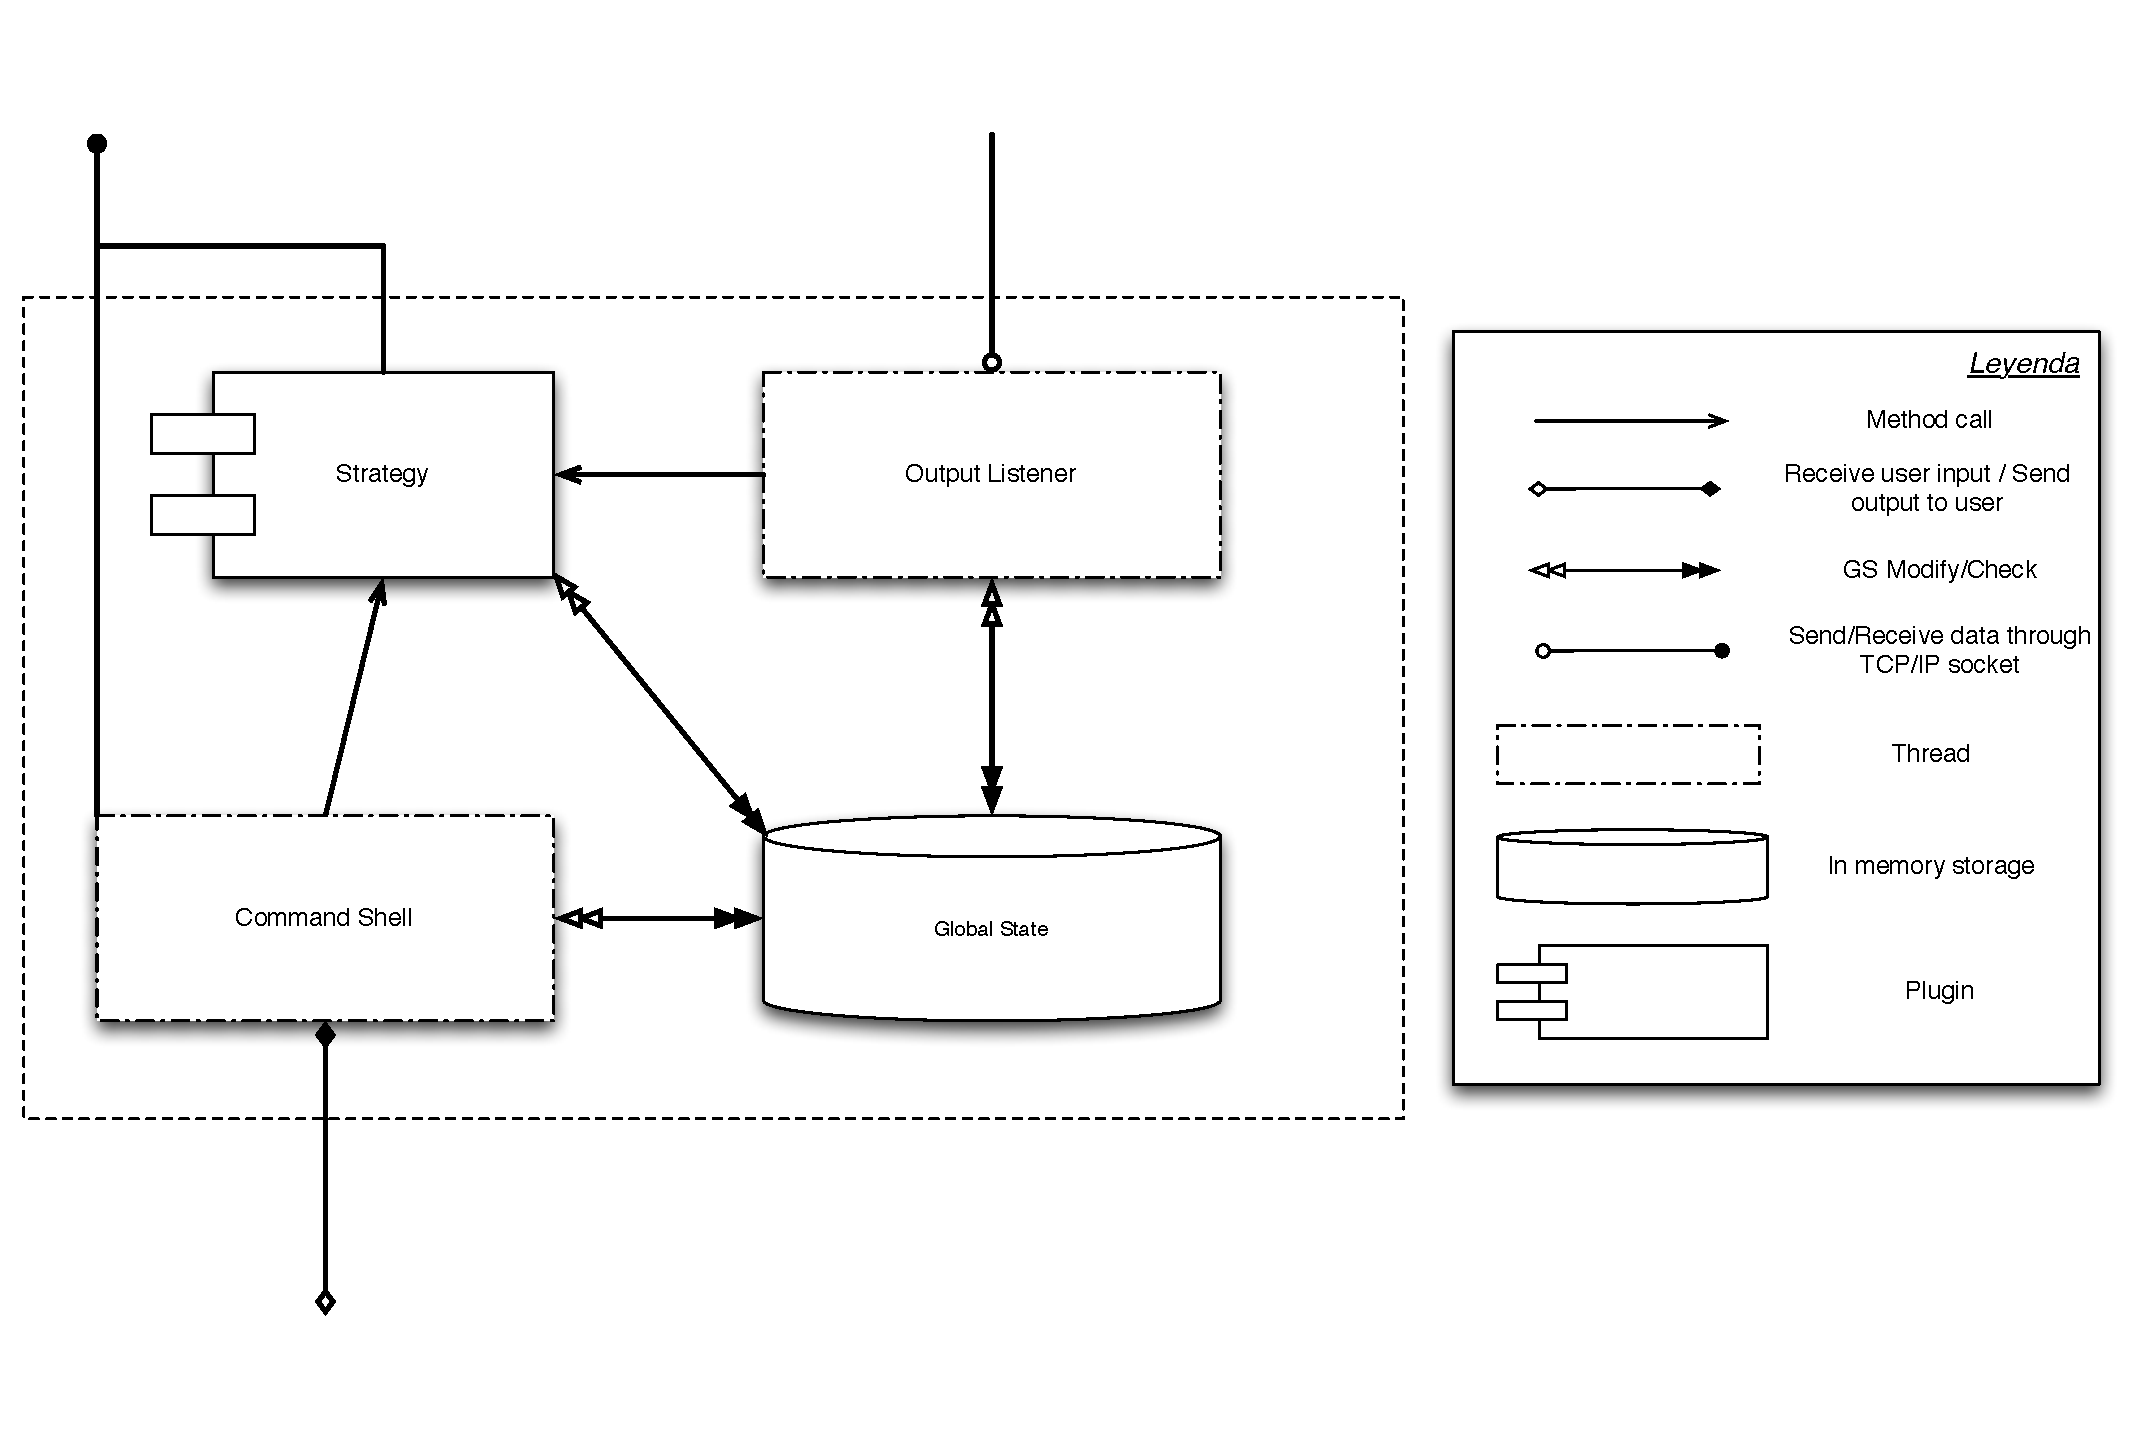
\includegraphics[scale=0.4]{graphs/frontend architecture}
\caption{Detalle de arquitectura del \fend}
\label{fig:frontend}
\end{figure}

\begin{wrapfigure}{r}{0.6\textwidth}
	\vspace{-3em}
	\begin{subfigure}{0.27\textwidth}
		\centering
		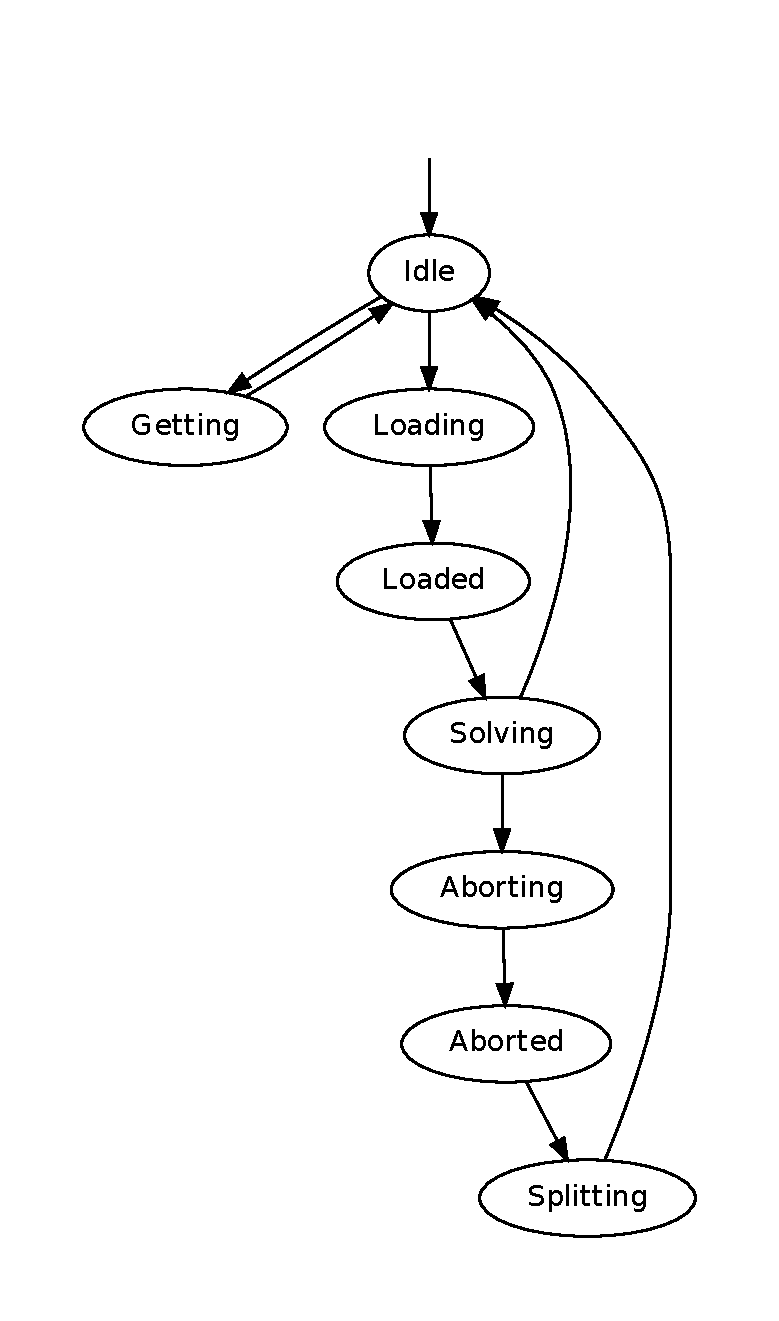
\includegraphics[scale=0.3]{graphs/workerstates}
		\caption{\emph{Workers}}
	\end{subfigure}
	\begin{subfigure}{0.27\textwidth}
		\centering
		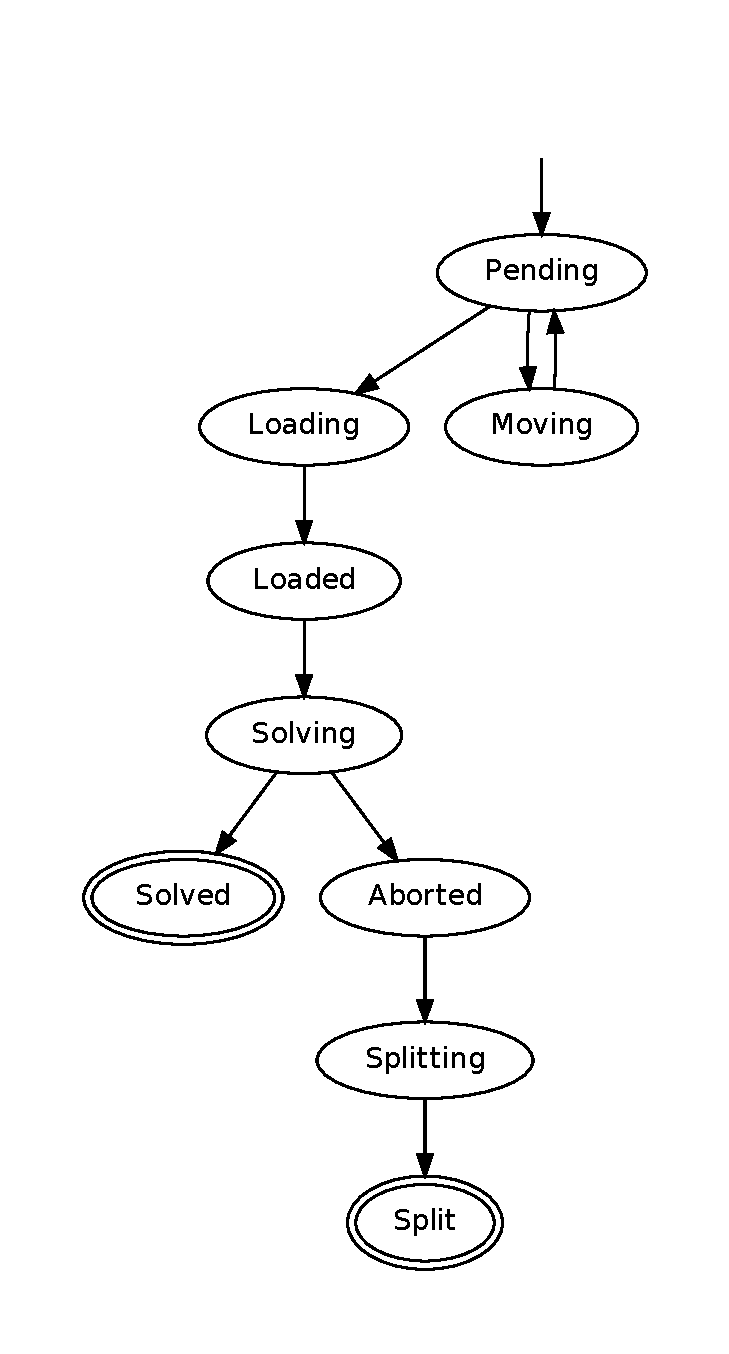
\includegraphics[scale=0.3]{graphs/taskstates}
		\caption{Tareas}
	\end{subfigure}
	\caption{Diagramas de estado en el tablero de control}
	\label{fig:states}
	\vspace{-1em}
\end{wrapfigure}

En la \fig\ref{fig:frontend} se esquematiza el diseño de componentes del
\fend. En esta figura se puede observar que el tablero de control proporciona
un modo doble de interacción con el \bend. Por un lado el tablero de control
es capaz de recibir comandos del usuario en \rt a través de una interfaz de
tipo consola. Estos comandos representan acciones a ser llevadas a cabo en el
\bend como ser indicar a un \w ocioso que cargue una nueva tarea, indicar a un
\w que se encuentra trabajando en un problema que aborte dicha ejecución,
mover una tarea desde un \w a otro, etc. Por otro lado, el tablero de control
posee también una \emph{estrategia} (intercambiable) que permite llevar a cabo
acciones automáticamente frente a determinados eventos. El \fend posee también
un componente que procesa permanentemente la información que llega desde el
\bend. 

Es importante observar que todos los componentes mencionados comparten un
estado global. Esto se debe a que, tal como se explicó en \ref{sec:backend},
el \bend no almacena el estado del sistema. Por lo tanto esta responsabilidad
recae en el \fend en la medida que este estado es necesario para poder tomar
decisiones ante los distintos eventos. El acceso concurrente a este estado
global nos obliga a introducir un mecanismo de sincronización entre los
distintos \threads de ejecución (\emph{locking}) que garantice la consistencia
del estado en todo momento. Hemos tenido el cuidado necesario para evitar que
el \emph{locking} atente contra la performance del componente en cuestión.

\begin{wrapfigure}{r}{.6\textwidth}
\vspace{-2em}
\begin{footnotesize}
\begin{lstlisting}[mathescape,language=Pascal,frame=single,label=lst:synchronouscmd,caption=Esquema de comando sincrónico]
DECIR_A $W$ que obtenga la tarea $T$
ESPERAR que tarea $T$ este en $W$
DECIR_A $W$ que cargue tarea $T$
ESPERAR que tarea $T$ este cargada
DECIR_A $W$ que comience a solvear $T$
\end{lstlisting}
\end{footnotesize}
\vspace{-3em}
\end{wrapfigure}

En la \fig\ref{fig:states} presentamos las máquinas de estado correspondientes
a los \ws y a las tareas. Estos diagramas esquematizan el estado que es
mantenido en el estado global del \fend. Una estrategia particular podría
requerir un estado más \emph{complejo} para tomar decisiones. Por ejemplo se
podría requerir mantener cierta información histórica respecto de la
ejecución. En tal caso queda bajo exclusiva responsabilidad de la estrategia
la implementación de las estructuras de datos y algoritmos necesarios para
dicha tarea.


\newcommand{\lst}{List.-}

\begin{wrapfigure}{r}{.6\textwidth}
\begin{footnotesize}
\begin{lstlisting}[language=Python,caption=Interfaz Strategy,label=lst:strategy]
class Strategy(object):
	def register_globalstate(globalstate)
	def register_socket(commandsocket)
	def on_init(worker)
	def on_createroot(worker, task)
	def on_init_finished(nworkers)
	def on_getfile(worker, task)
	def on_file(worker, task)
	def on_load(worker, task)
	def on_unsat(worker, task)
	def on_sat(worker, task, modelstr)
	def on_abort(worker, task)
	def on_split_newtask(worker, newtask)
	def on_split_finished(worker, 
	                      parenttask, 
	                      nchildren)
	def on_shutdown()
\end{lstlisting}
\end{footnotesize}
\end{wrapfigure}

En cuanto a las estrategias, se siguió un modelo reactivo (\emph{eventos}).
Esto se debió en primera instancia a la dificultad de ejecutar secuencias de
comandos de forma sincrónica. Por ejemplo, si quisiéramos implementar la
obtención automática de una nueva tarea cuando un \w se queda sin tareas
pendientes y quisiéramos además que el \w comenzara a \solvear dicha tarea en
el momento en el que la misma esté disponible, deberíamos implementar un
algoritmo similar al expuesto en \lst\ref{lst:synchronouscmd}. El problema en
este algoritmo se encuentra en las líneas que comienzan con la palabra clave
\texttt{ESPERAR} ya que no es aceptable que la consola de comandos o la
estrategia se bloqueen a la espera de un evento que puede tardar una cantidad
arbitraria de tiempo en ocurrir. Esto se debe principalmente a que en el
transcurso de esa cantidad arbitraria de tiempo el \fend recibiría una
cantidad de información desde el \bend (por ejemplo el hecho de que otro \w
terminó de \solvear el subproblema en el que estaba trabajando) que podría
requerir que se tomen acciones con el fin de mantener el sistema funcionando
eficientemente. Sin embargo estas acciones no podrían ser tomadas porque el
\fend se encontraría bloqueado esperando a que un evento particular de un \w
particular ocurra. Ante este escenario optamos por un modelo de eventos que
presentamos en el \lst\ref{lst:strategy}. Esta interfaz modela el conjunto de
eventos que pueden ocurrir. Una estrategia particular debe implementar dicha
interfaz de modo de poder responder ante estos eventos.

\subsection{La estrategia implementada}



\begin{itemize}
	\item Si idle se parte el más viejo
	\item La próxima a resolver es:
		\begin{itemize}
			\item Si no tengo tareas locales:
				\begin{itemize}
					\item Bajo la tarea que corresponde por BFS +
					\item $\frac{\sharp tasks}{\sharp workers}$ del que más tiene (límite 10)
				\end{itemize}
			\item Si tengo: Agarro la que corresponde por BFS
		\end{itemize}
	\item Parto cuando la frecuencia de $\sharp UNSATs/_s$
	\item Detalles:
	\begin{itemize}
		\item Target de UNSATs por esgundo
		\item Frecuencia de checkeo
		\item Tamaño ventana
	\end{itemize}
\end{itemize}

\subsection{Decisiones que vale la pena seguir investigando}

\section{Resultados experimentales}

\begin{table}[h]\tiny
	\begin{tabular}{lrrrrrr}
		\toprule
		problem	&	scope	&	sequential runtime	&	parallel walltime	&	parallel overhead	&	speedup	&	efficiency \\
		\cmidrule(r){1-7}
		Pamela	&	8	&	308.26	&	60.46	&	3561.23	&	5.10x	&	0.08 \\
		Pamela	&	9	&	76168.16	&	407.34	&	-50098.63	&	186.99x	&	2.92 \\
		Pamela	&	10	&		&		&	0.00	&		&	 \\
		\cmidrule(r){1-7}
		Closure	&	11	&	749.65	&	291.28	&	17891.95	&	2.57x	&	0.04 \\
		Closure	&	12	&	3983.36	&	1914.45	&	118541.30	&	2.08x	&	0.03 \\
		Closure	&	13	&		&		&	0.00	&		&	 \\
		\cmidrule(r){1-7}
		MarkGC Soundness2	&	9	&	217.31	&	200.85	&	12637.31	&	1.08x	&	0.02 \\
		MarkGC Soundness2	&	10	&	2855.3	&	1376.89	&	85265.47	&	2.07x	&	0.03 \\
		\bottomrule
	\end{tabular}
	\caption{Tiempo de ejecución (en segundos) distribuido vs. secuencial}
	\todo[inline]{Resultados parciales. Completar con todos los experimentos}
\end{table}